% Created by tikzDevice version 0.12.6 on 2024-01-04 11:14:35
% !TEX encoding = UTF-8 Unicode
\documentclass[tikz]{standalone}

\nonstopmode

\usepackage[fontset=fandol]{ctex}
\usepackage{amsfonts,mathrsfs,amssymb}
\begin{document}

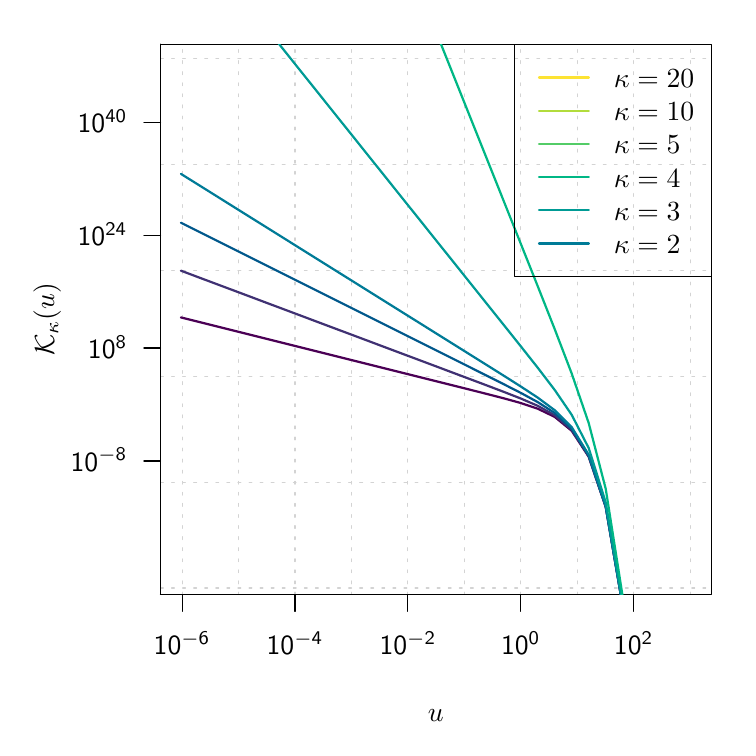
\begin{tikzpicture}[x=1pt,y=1pt]
\definecolor{fillColor}{RGB}{255,255,255}
\path[use as bounding box,fill=fillColor,fill opacity=0.00] (0,0) rectangle (252.94,252.94);
\begin{scope}
\path[clip] ( 48.00, 48.00) rectangle (246.94,246.94);
\definecolor{drawColor}{RGB}{211,211,211}

\path[draw=drawColor,line width= 0.4pt,dash pattern=on 1pt off 3pt ,line join=round,line cap=round] ( 55.79, 48.00) -- ( 55.79,246.94);

\path[draw=drawColor,line width= 0.4pt,dash pattern=on 1pt off 3pt ,line join=round,line cap=round] ( 76.19, 48.00) -- ( 76.19,246.94);

\path[draw=drawColor,line width= 0.4pt,dash pattern=on 1pt off 3pt ,line join=round,line cap=round] ( 96.58, 48.00) -- ( 96.58,246.94);

\path[draw=drawColor,line width= 0.4pt,dash pattern=on 1pt off 3pt ,line join=round,line cap=round] (116.98, 48.00) -- (116.98,246.94);

\path[draw=drawColor,line width= 0.4pt,dash pattern=on 1pt off 3pt ,line join=round,line cap=round] (137.38, 48.00) -- (137.38,246.94);

\path[draw=drawColor,line width= 0.4pt,dash pattern=on 1pt off 3pt ,line join=round,line cap=round] (157.78, 48.00) -- (157.78,246.94);

\path[draw=drawColor,line width= 0.4pt,dash pattern=on 1pt off 3pt ,line join=round,line cap=round] (178.17, 48.00) -- (178.17,246.94);

\path[draw=drawColor,line width= 0.4pt,dash pattern=on 1pt off 3pt ,line join=round,line cap=round] (198.57, 48.00) -- (198.57,246.94);

\path[draw=drawColor,line width= 0.4pt,dash pattern=on 1pt off 3pt ,line join=round,line cap=round] (218.97, 48.00) -- (218.97,246.94);

\path[draw=drawColor,line width= 0.4pt,dash pattern=on 1pt off 3pt ,line join=round,line cap=round] (239.37, 48.00) -- (239.37,246.94);

\path[draw=drawColor,line width= 0.4pt,dash pattern=on 1pt off 3pt ,line join=round,line cap=round] ( 48.00, 50.48) -- (246.94, 50.48);

\path[draw=drawColor,line width= 0.4pt,dash pattern=on 1pt off 3pt ,line join=round,line cap=round] ( 48.00, 88.72) -- (246.94, 88.72);

\path[draw=drawColor,line width= 0.4pt,dash pattern=on 1pt off 3pt ,line join=round,line cap=round] ( 48.00,126.97) -- (246.94,126.97);

\path[draw=drawColor,line width= 0.4pt,dash pattern=on 1pt off 3pt ,line join=round,line cap=round] ( 48.00,165.22) -- (246.94,165.22);

\path[draw=drawColor,line width= 0.4pt,dash pattern=on 1pt off 3pt ,line join=round,line cap=round] ( 48.00,203.46) -- (246.94,203.46);

\path[draw=drawColor,line width= 0.4pt,dash pattern=on 1pt off 3pt ,line join=round,line cap=round] ( 48.00,241.71) -- (246.94,241.71);
\end{scope}
\begin{scope}
\path[clip] (  0.00,  0.00) rectangle (252.94,252.94);
\definecolor{drawColor}{RGB}{0,0,0}

\path[draw=drawColor,line width= 0.4pt,line join=round,line cap=round] ( 48.00, 48.00) --
	(246.94, 48.00) --
	(246.94,246.94) --
	( 48.00,246.94) --
	cycle;
\end{scope}
\begin{scope}
\path[clip] (  0.00,  0.00) rectangle (252.94,252.94);
\definecolor{drawColor}{RGB}{0,0,0}

\node[text=drawColor,anchor=base,inner sep=0pt, outer sep=0pt, scale=  1.00] at (147.47,  2.40) {$u$};

\node[text=drawColor,rotate= 90.00,anchor=base,inner sep=0pt, outer sep=0pt, scale=  1.00] at (  9.60,147.47) {$\mathcal{K}_{\kappa}(u)$};
\end{scope}
\begin{scope}
\path[clip] (  0.00,  0.00) rectangle (252.94,252.94);
\definecolor{drawColor}{RGB}{0,0,0}

\path[draw=drawColor,line width= 0.4pt,line join=round,line cap=round] ( 48.00, 48.00) -- (218.97, 48.00);

\path[draw=drawColor,line width= 0.4pt,line join=round,line cap=round] ( 55.79, 48.00) -- ( 55.79, 42.00);

\path[draw=drawColor,line width= 0.4pt,line join=round,line cap=round] ( 96.58, 48.00) -- ( 96.58, 42.00);

\path[draw=drawColor,line width= 0.4pt,line join=round,line cap=round] (137.38, 48.00) -- (137.38, 42.00);

\path[draw=drawColor,line width= 0.4pt,line join=round,line cap=round] (178.17, 48.00) -- (178.17, 42.00);

\path[draw=drawColor,line width= 0.4pt,line join=round,line cap=round] (218.97, 48.00) -- (218.97, 42.00);

\node[text=drawColor,anchor=base,inner sep=0pt, outer sep=0pt, scale=  1.00] at ( 55.79, 26.40) {$\mathsf{10^{-6}}$};

\node[text=drawColor,anchor=base,inner sep=0pt, outer sep=0pt, scale=  1.00] at ( 96.58, 26.40) {$\mathsf{10^{-4}}$};

\node[text=drawColor,anchor=base,inner sep=0pt, outer sep=0pt, scale=  1.00] at (137.38, 26.40) {$\mathsf{10^{-2}}$};

\node[text=drawColor,anchor=base,inner sep=0pt, outer sep=0pt, scale=  1.00] at (178.17, 26.40) {$\mathsf{10^{0}}$};

\node[text=drawColor,anchor=base,inner sep=0pt, outer sep=0pt, scale=  1.00] at (218.97, 26.40) {$\mathsf{10^{2}}$};

\path[draw=drawColor,line width= 0.4pt,line join=round,line cap=round] ( 48.00, 96.37) -- ( 48.00,246.95);

\path[draw=drawColor,line width= 0.4pt,line join=round,line cap=round] ( 48.00, 96.37) -- ( 42.00, 96.37);

\path[draw=drawColor,line width= 0.4pt,line join=round,line cap=round] ( 48.00,137.17) -- ( 42.00,137.17);

\path[draw=drawColor,line width= 0.4pt,line join=round,line cap=round] ( 48.00,177.96) -- ( 42.00,177.96);

\path[draw=drawColor,line width= 0.4pt,line join=round,line cap=round] ( 48.00,218.76) -- ( 42.00,218.76);

\node[text=drawColor,anchor=base east,inner sep=0pt, outer sep=0pt, scale=  1.00] at ( 36.00, 92.74) {$\mathsf{10^{-8}}$};

\node[text=drawColor,anchor=base east,inner sep=0pt, outer sep=0pt, scale=  1.00] at ( 36.00,133.54) {$\mathsf{10^{8}}$};

\node[text=drawColor,anchor=base east,inner sep=0pt, outer sep=0pt, scale=  1.00] at ( 36.00,174.33) {$\mathsf{10^{24}}$};

\node[text=drawColor,anchor=base east,inner sep=0pt, outer sep=0pt, scale=  1.00] at ( 36.00,215.13) {$\mathsf{10^{40}}$};
\end{scope}
\begin{scope}
\path[clip] ( 48.00, 48.00) rectangle (246.94,246.94);
\definecolor{drawColor}{RGB}{75,0,85}

\path[draw=drawColor,line width= 0.8pt,line join=round,line cap=round] ( 55.37,148.24) --
	( 61.51,146.70) --
	( 67.65,145.17) --
	( 73.79,143.63) --
	( 79.93,142.10) --
	( 86.07,140.56) --
	( 92.21,139.03) --
	( 98.35,137.49) --
	(104.49,135.96) --
	(110.63,134.42) --
	(116.77,132.89) --
	(122.91,131.35) --
	(129.05,129.82) --
	(135.19,128.28) --
	(141.33,126.75) --
	(147.47,125.21) --
	(153.61,123.68) --
	(159.75,122.14) --
	(165.89,120.59) --
	(172.03,119.01) --
	(178.17,117.31) --
	(184.31,115.25) --
	(190.45,112.29) --
	(196.59,107.26) --
	(202.73, 97.89) --
	(208.88, 79.73) --
	(215.02, 43.88) --
	(221.16,-27.39) --
	(227.30,-169.51) --
	(233.44,-453.38);
\definecolor{drawColor}{RGB}{64,49,115}

\path[draw=drawColor,line width= 0.8pt,line join=round,line cap=round] ( 55.37,165.13) --
	( 61.51,162.82) --
	( 67.65,160.52) --
	( 73.79,158.22) --
	( 79.93,155.92) --
	( 86.07,153.61) --
	( 92.21,151.31) --
	( 98.35,149.01) --
	(104.49,146.70) --
	(110.63,144.40) --
	(116.77,142.10) --
	(122.91,139.80) --
	(129.05,137.49) --
	(135.19,135.19) --
	(141.33,132.89) --
	(147.47,130.59) --
	(153.61,128.28) --
	(159.75,125.98) --
	(165.89,123.67) --
	(172.03,121.34) --
	(178.17,118.94) --
	(184.31,116.29) --
	(190.45,112.88) --
	(196.59,107.58) --
	(202.73, 98.06) --
	(208.88, 79.82) --
	(215.02, 43.93) --
	(221.16,-27.36) --
	(227.30,-169.50) --
	(233.44,-453.37);
\definecolor{drawColor}{RGB}{0,88,139}

\path[draw=drawColor,line width= 0.8pt,line join=round,line cap=round] ( 55.37,182.46) --
	( 61.51,179.39) --
	( 67.65,176.32) --
	( 73.79,173.25) --
	( 79.93,170.18) --
	( 86.07,167.11) --
	( 92.21,164.04) --
	( 98.35,160.97) --
	(104.49,157.90) --
	(110.63,154.83) --
	(116.77,151.76) --
	(122.91,148.69) --
	(129.05,145.62) --
	(135.19,142.55) --
	(141.33,139.48) --
	(147.47,136.41) --
	(153.61,133.34) --
	(159.75,130.27) --
	(165.89,127.19) --
	(172.03,124.10) --
	(178.17,120.97) --
	(184.31,117.64) --
	(190.45,113.70) --
	(196.59,108.03) --
	(202.73, 98.30) --
	(208.88, 79.94) --
	(215.02, 43.99) --
	(221.16,-27.33) --
	(227.30,-169.49) --
	(233.44,-453.36);
\definecolor{drawColor}{RGB}{0,123,151}

\path[draw=drawColor,line width= 0.8pt,line join=round,line cap=round] ( 55.37,200.11) --
	( 61.51,196.28) --
	( 67.65,192.44) --
	( 73.79,188.60) --
	( 79.93,184.76) --
	( 86.07,180.93) --
	( 92.21,177.09) --
	( 98.35,173.25) --
	(104.49,169.41) --
	(110.63,165.57) --
	(116.77,161.74) --
	(122.91,157.90) --
	(129.05,154.06) --
	(135.19,150.22) --
	(141.33,146.39) --
	(147.47,142.55) --
	(153.61,138.71) --
	(159.75,134.87) --
	(165.89,131.03) --
	(172.03,127.18) --
	(178.17,123.29) --
	(184.31,119.26) --
	(190.45,114.70) --
	(196.59,108.59) --
	(202.73, 98.59) --
	(208.88, 80.09) --
	(215.02, 44.06) --
	(221.16,-27.30) --
	(227.30,-169.47) --
	(233.44,-453.35);
\definecolor{drawColor}{RGB}{0,155,149}

\path[draw=drawColor,line width= 0.8pt,line join=round,line cap=round] ( 55.37,291.36) --
	( 61.51,283.69) --
	( 67.65,276.01) --
	( 73.79,268.34) --
	( 79.93,260.66) --
	( 86.07,252.98) --
	( 92.21,245.31) --
	( 98.35,237.63) --
	(104.49,229.96) --
	(110.63,222.28) --
	(116.77,214.61) --
	(122.91,206.93) --
	(129.05,199.26) --
	(135.19,191.58) --
	(141.33,183.91) --
	(147.47,176.23) --
	(153.61,168.56) --
	(159.75,160.88) --
	(165.89,153.20) --
	(172.03,145.52) --
	(178.17,137.82) --
	(184.31,130.06) --
	(190.45,122.02) --
	(196.59,113.03) --
	(202.73,101.03) --
	(208.88, 81.36) --
	(215.02, 44.70) --
	(221.16,-26.97) --
	(227.30,-169.31) --
	(233.44,-453.27);
\definecolor{drawColor}{RGB}{0,183,133}

\path[draw=drawColor,line width= 0.8pt,line join=round,line cap=round] ( 55.37,481.93) --
	( 61.51,466.58) --
	( 67.65,451.23) --
	( 73.79,435.88) --
	( 79.93,420.53) --
	( 86.07,405.18) --
	( 92.21,389.83) --
	( 98.35,374.48) --
	(104.49,359.12) --
	(110.63,343.77) --
	(116.77,328.42) --
	(122.91,313.07) --
	(129.05,297.72) --
	(135.19,282.37) --
	(141.33,267.02) --
	(147.47,251.67) --
	(153.61,236.32) --
	(159.75,220.97) --
	(165.89,205.62) --
	(172.03,190.26) --
	(178.17,174.90) --
	(184.31,159.51) --
	(190.45,143.98) --
	(196.59,127.95) --
	(202.73,110.06) --
	(208.88, 86.29) --
	(215.02, 47.26) --
	(221.16,-25.68) --
	(227.30,-168.66) --
	(233.44,-452.95);
\definecolor{drawColor}{RGB}{0,0,0}

\path[draw=drawColor,line width= 0.4pt,line join=round,line cap=round] (175.78,246.94) rectangle (246.94,162.94);
\definecolor{drawColor}{RGB}{253,227,51}

\path[draw=drawColor,line width= 0.8pt,line join=round,line cap=round] (184.78,234.94) -- (202.78,234.94);
\definecolor{drawColor}{RGB}{178,220,60}

\path[draw=drawColor,line width= 0.8pt,line join=round,line cap=round] (184.78,222.94) -- (202.78,222.94);
\definecolor{drawColor}{RGB}{83,204,103}

\path[draw=drawColor,line width= 0.8pt,line join=round,line cap=round] (184.78,210.94) -- (202.78,210.94);
\definecolor{drawColor}{RGB}{0,183,133}

\path[draw=drawColor,line width= 0.8pt,line join=round,line cap=round] (184.78,198.94) -- (202.78,198.94);
\definecolor{drawColor}{RGB}{0,155,149}

\path[draw=drawColor,line width= 0.8pt,line join=round,line cap=round] (184.78,186.94) -- (202.78,186.94);
\definecolor{drawColor}{RGB}{0,123,151}

\path[draw=drawColor,line width= 0.8pt,line join=round,line cap=round] (184.78,174.94) -- (202.78,174.94);
\definecolor{drawColor}{RGB}{0,0,0}

\node[text=drawColor,anchor=base west,inner sep=0pt, outer sep=0pt, scale=  1.00] at (211.78,231.31) {$\kappa=20$};

\node[text=drawColor,anchor=base west,inner sep=0pt, outer sep=0pt, scale=  1.00] at (211.78,219.31) {$\kappa=10$};

\node[text=drawColor,anchor=base west,inner sep=0pt, outer sep=0pt, scale=  1.00] at (211.78,207.31) {$\kappa=5$};

\node[text=drawColor,anchor=base west,inner sep=0pt, outer sep=0pt, scale=  1.00] at (211.78,195.31) {$\kappa=4$};

\node[text=drawColor,anchor=base west,inner sep=0pt, outer sep=0pt, scale=  1.00] at (211.78,183.31) {$\kappa=3$};

\node[text=drawColor,anchor=base west,inner sep=0pt, outer sep=0pt, scale=  1.00] at (211.78,171.31) {$\kappa=2$};
\end{scope}
\end{tikzpicture}

\end{document}
